\newcommand{\entrynode}[0]{\ensuremath{\mathbf{entry}}}
\newcommand{\exitnode}[0]{\ensuremath{\mathbf{exit}}}
\section{Refined block sinking and loop nesting forests}
\label{sec:part1:semantics:LNF}
As discussed when outlining $\lambda$-dropping, block sinking is
governed by the dominance relation between basic blocks. Thus, a
typical dominance tree with root $b$ and subtrees rooted at
$b_1,\ldots,b_n$ is most naturally represented as a block of function
declarations for the $f_i$, nested inside the declaration of $f$:
\begin{equation}
\label{sec:SSA:functiondeclarationblock}
\begin{array}{l}
  \mathtt{function}\ f (\ldots)= 
  \mathtt{let} \ldots (*\ \mathit{body\ of}\ b\ \mathit{*)}\ldots \mathtt{in}\\
  \quad \begin{array}{l}
          \begin{array}{rcl}
            \mathtt{function}\ f_1(\ldots) & = & e_1\
                  (*\ \mathit{body\ of}\ b_1, \mathit{with\ calls\ to}\ 
                      b, b_i\ \mathit{*)}\\
             : \\
            \mathtt{and}\ f_n(\ldots) & = & e_n
                  (*\ \mathit{body\ of}\ b_n, \mathit{with\ calls\ to}\ 
                      b, b_i\ \mathit{*)}
          \end{array}\\
          \mathtt{in} \ldots (*\ b\mathit{'s\ calls\ to}\ b, b_i\ \mathit{*)} 
            \ldots\ \mathtt{end}
        \end{array}
  \end{array}
\end{equation}
By exploiting additional control-flow structure between the $b_i$, it
is, however, possible to obtain refined placements, namely placements
that correspond to notions of \emph{loop nesting forests} that have
been identified in the SSA literature.

These refinements arise if we enrich the above dominance tree by
adding arrows $b_i \to b_j$ whenever the CFG contains a directed
edge from one of $b_i$'s dominance successors (i.e.~the descendants of
$b_i$ in the dominance tree) to $b_j$.

In the case of a \emph{reducible} CFG, the resulting graph contains
only trivial loops. Ignoring these self-loops, we perform a
post-order-DFS (or more generally a reverse topological ordering)
amongst the $b_i$ and stagger the function declarations according to
the resulting order.
\begin{figure}
\begin{center}
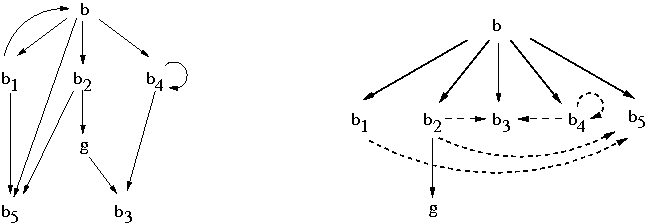
\includegraphics[scale=0.5]{shortloopAnalysis1}
\end{center}
\caption{\label{FigShortLoopAnalysis1ReducibleGraph} Example placement
  for reducible flow graphs. (a) control-flow graph (b) overlay of CFG
  (dashed edges) arcs between dominatees onto dominance graph (solid
  edges) }
\end{figure}
As an example, consider the CFG in
Figure~\ref{FigShortLoopAnalysis1ReducibleGraph}(a) and its enriched
dominance tree shown in
Figure\ref{FigShortLoopAnalysis1ReducibleGraph}(b). A possible (but
not unique) ordering of $b$'s children is $[b_5,b_1,b_3,b_2,b_4]$,
resulting in the nesting shown in code~(\ref{FunctionalCascadeFun}).
\begin{equation}
\label{FunctionalCascadeFun}
\begin{array}{l}
  \mathtt{function}\ f (\ldots)= 
  \mathtt{let} \ldots (*\ \mathit{body\ of}\ f\ *)\ldots \mathtt{in}\\
  \quad \begin{array}{l}
          \mathtt{function}\ f_5(\ldots) = e_5\\ \mathtt{in}\  
          \begin{array}[t]{l}
            \mathtt{function}\ f_1(\ldots) = e_1\ 
                 (*\ \mathit{contains\ calls\ to}\ f\ \mathit{and}\ f_5\ *) \\
            \mathtt{in}\ 
            \begin{array}[t]{l}
              \mathtt{function}\ f_3(\ldots) = e_3\\ \mathtt{in}\ 
              \begin{array}[t]{l}
                \mathtt{function}\ f_2(\ldots) =\\
                \qquad
                  \begin{array}[t]{l}
                    \mathtt{let} \ldots\ (*\ \mathit{body\ of}\ f_2\ *)\ldots\\
                    \mathtt{in}\
                      \begin{array}[t]{l}
                        \mathtt{function}\ g(\ldots) = e_g\
                           (*\ \mathit{contains\ call\ to}\ f_3\ *)\\ 
                        \mathtt{in}\   \ldots 
                              (*\ \mathit{calls\ to\ f_5}\ \mathit{and}\ g\ *)
                        \ldots \mathtt{end}
                     \end{array}\\
                   \end{array}\\ 
                \mathtt{in}\
                \begin{array}[t]{l}
                  \mathtt{function}\ f_4(\ldots) = e_4\
                    (*\ \mathit{contains\ calls\ to}\ f_3\ 
                        \mathit{and}\ f_4\ *) \\
                   \mathtt{in} \ldots 
                      (*\ \mathit{calls\ to}\ f_1, f_2, f_4, f_5\ *)
                   \ldots \mathtt{end}
                \end{array}
              \end{array}
            \end{array}
          \end{array}
        \end{array}
  \end{array}
\end{equation}
The code respects the dominance relationship in much the same way as
the naive placement, but additionally makes $f_1$ inacessible
from within $e_5$, and makes $f_3$ inaccessible from within $f_1$ or
$f_5$. As the reordering does not move function declarations
\emph{inside} each other (in particular: no function declaration is
brought into or moved out of the scope of the formal parameters of any
other function) the reordering does not affect the potential to
subsequently perform parameter dropping.

A further improvement is obtained if functions are declared using
$\lambda$-abstraction. This enables us not only to syntactically
distinguish between loops and non-recursive control-flow structures
using the distinction between $\mathtt{let}$ and $\mathtt{letrec}$
present in many functional languages, but also to further restrict the
visibility of function names. Indeed, while $b_3$ is immediately
dominated by $b$ in the above example, its only control-flow
predecessors are $b_2/g$ and $b_4$. We would hence like to make the
declaration of $f_3$ local to the \emph{tuple} $(f_2, f_4)$,
i.e.~invisible to $f$.  This can be achieved by combining
$\mathtt{let}$/$\mathtt{letrec}$ binding with pattern matching, if we
insert the shared declaration of $f_3$
\emph{between} the declaration of the names $f_2$ and $f_4$ and the
$\lambda$-bindings of their formal parameters $p_i$:
\begin{equation}
\label{FuntionalCascadeFunLambda}
\begin{array}{l}
  \mathtt{letrec}\ f = \lambda\; p.\;
  \mathtt{let} \ldots (*\ \mathit{body\ of}\ f\ *)\ldots \mathtt{in}\\
  \quad \begin{array}{l}
          \mathtt{let}\ f_5 = \lambda\; p_5.\; e_5\\ \mathtt{in}\  
          \begin{array}[t]{l}
            \mathtt{let}\ f_1 = \lambda\;  p_1.\; e_1\ 
                 (* \mathit{contains\ calls\ to}\ f\ \mathit{and}\ f_5\ *) \\
            \mathtt{in}\ 
            \begin{array}[t]{l}
               \mathtt{letrec}\ (f_2, f_4) =\\ 
               \quad 
                 \begin{array}{l}
                   \mathtt{let}\ f_3 = \lambda\; p_3.\; e_3\\ \mathtt{in}\ 
                   \begin{array}[t]{l}
                   (\lambda\; p_2.\; 
                       \begin{array}[t]{l}
                         \mathtt{let} \ldots 
                            (*\ \mathit{body\ of}\ f_2\ *)\ldots
                         \mathtt{in}\\
                         \quad \begin{array}{l}
                           \mathtt{let}\ g = \lambda\; p_g.\; e_g\
                              (*\ \mathit{contains\ call\ to}\ f_3\ *)\\ 
                           \mathtt{in}\   \ldots 
                                 (*\ \mathit{calls\ to}\ f_5\ 
                                     \mathit{and}\ g\ *)
                           \ldots \mathtt{end},
                         \end{array}
                       \end{array}\\
                    \; \lambda\; p_4.\; e_4\
                       (*\ \mathit{contains\ calls\ to}\ f_3\ 
                           \mathit{and}\ f_4\ *))
                  \end{array}\\
               \mathtt{end}\ (*\ \mathit{declaration\ of\ tuple}\ (f_2,f_4)\
                                 \mathit{ends\ here}\ *) 
            \end{array}\\
            \mathtt{in} \ldots 
               (*\ \mathit{calls\ to}\ f_1, f_2, f_4, f_5\ *)
                 \ldots \mathtt{end}
            \end{array}
          \end{array}
        \end{array}
  \end{array}
\end{equation}
The recursiveness of $f_4$ is inherited by the function pair
$(f_2,f_4)$ but $f_3$ remains non-recursive. In general, the role of
$f_3$ is played by any merge point $b_i$ that is not directly called
from the dominator node $b$.

In the case of \emph{irreducible} CFG's, the enriched dominance tree
is no longer acyclic, even when self-loops are ignored. In this case,
the functional representation not only depends on the chosen DFS order
but additionally on the partitioning of the enriched graph into loops.
As each loop forms a \emph{strongly connected component} (SCC),
different partitionings are possible, corresponding to different
notions of \emph{loop nesting forests} (LNF's). Of the various LNF
strategies proposed in the SSA-literature, the scheme introduced by
Steensgaard is particularly appealing from a functional perspective.

%\begin{description}
%\item[Steensgaard's] 
In Steengaard's notion of loops, the headers $H$ of a loop $L=(B,H)$
are precisely the entry nodes of its body $B$, i.e.~those nodes in $B$
that have a predecessor outside of $B$.  For example, the CFG $G_0$
shown in Figure~\ref{FigLoopAnalysisRamalingamSteensgaardConstruction}
contains the outer loop $L_0 = (\{u,v,w,x\}, \{u,v\})$, whose
constituents $B_0$ are determined as the maximal SCC of
$G_0$. Removing $L_0$'s back-edges (i.e.~edges from $B_0$ to $H_0$)
from $G_0$ yields $G_1$, whose (only) SCC determines a further, inner,
loop $L_1 = (\{w,x\},
\{w,x\})$. Removing $L_1$'s back-edges from $G_1$ results in the
acyclic $G_2$, terminating the process.

 \begin{figure}
    \begin{center}
    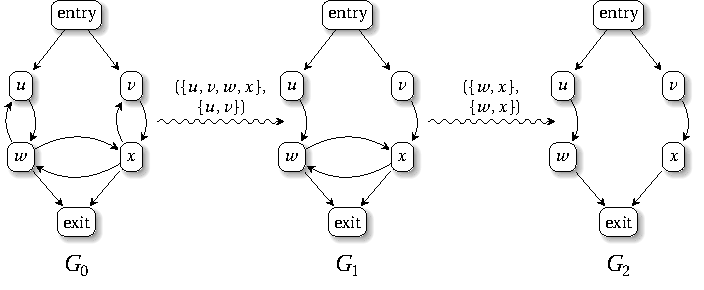
\includegraphics[scale=0.3]{RamalingamSteensgaardConstruction}
    \end{center}
    \caption{\label{FigLoopAnalysisRamalingamSteensgaardConstruction} 
       Illustration
       of Steensgaard's construction of loop nesting forests (from
       Ramalingam~\cite{DBLP:journals/toplas/Ramalingam02}):
       Iterative construction of graphs $G_1$ and $G_2$.}
  \end{figure} 

Figure~\ref{FigLoopAnalysisRamalingamSteensgaardOverlayAndANF}(a)
shows the CFG-enriched dominance tree of $G_0$. The body of loop $L_0$
is easily identified as the maximal SCC, and likewise the body of
$L_1$ once the cycles $(u, w)$ and $(x,v)$ are broken by the removal
of $L_0$'s backdeges $w \to u$ and $x \to v$.

The LNF resulting from Steensgaard's contruction is shown in
Figure~\ref{FigLoopAnalysisRamalingamSteensgaardOverlayAndANF}(b). Loops
are drawn as ellipsis that are decorated with the appropriate header
nodes, and are nested in accordance with the containment relation $B_1
\subset B_0$ between the bodies.

%  \begin{figure}
%    \begin{center}
%    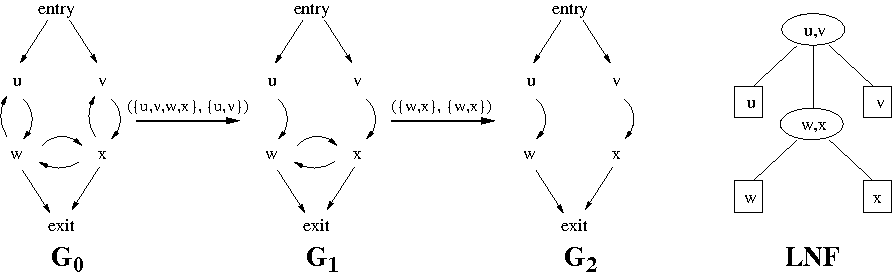
\includegraphics[scale=0.4]{RamalingamSteensgaard}
%    \end{center}
%    \caption{\label{FigLoopAnalysisRamalingamSteensgaard} 
%       Illustration
%       of Steensgaard's construction of loop nesting forests (from
%       Ramalingam~\cite{DBLP:journals/toplas/Ramalingam02}). 
%       (a) Iterative construction of graphs $G_1$ and $G_2$; 
%       (b) resulting loop nesting forest.}
%  \end{figure} 
  \begin{figure}
    \begin{center}
    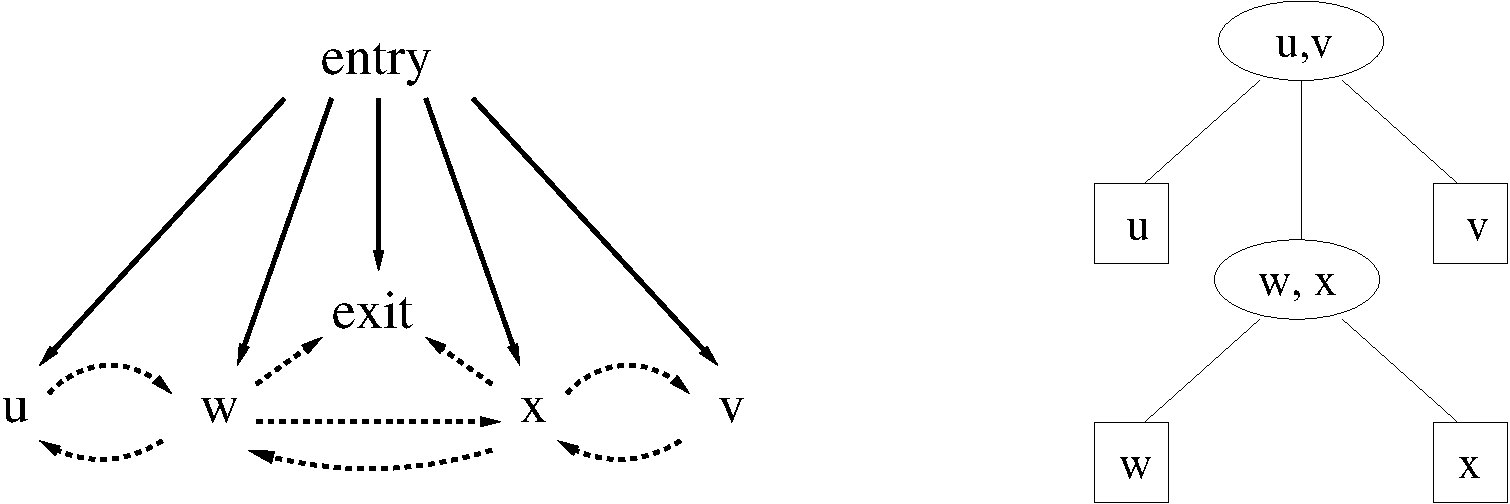
\includegraphics[scale=0.4]{RamalingamSteensgaardOverlayAndLNF}
    \end{center}
    \caption{\label{FigLoopAnalysisRamalingamSteensgaardOverlayAndANF} 
       Illustration
       of Steensgaard's construction of loop nesting forests: 
       (a) CFG-enriched dominance tree;
       (b) resulting loop nesting forest.}
  \end{figure} 

  In the functional representation, a loop $L=(B,H)$ with headers
  $H=\{h_1,\ldots,h_n\}$ yields a function declaration block for
  functions $h_1,\ldots,h_n$, with private declarations for the
  non-headers from $B \setminus H$. In our example, loop $L_0$
  provides entry points for the headers $u$ and $v$ but not for its
  non-headers $w$ and $x$.  Instead, the loop comprised of the latter
  nodes, $L_1$, is nested inside the definition of $L_0$, in
  accordance with the LNF.
  \begin{equation}
    \label{FunctionalSteensgaard}
     \begin{array}{l}
       \mathtt{function}\ \entrynode (\ldots)=\\ 
       \quad \mathtt{let} \ldots (*\ \mathit{body\ of\ \entrynode}\ *)\ldots\\
       \quad \mathtt{in}\ 
         \begin{array}[t]{l}
           (*\ \mathit{Define\ outer\ loop}\ L_0,\ 
               \mathit{with\ headers}\ u, v\ *)\\
           \mathtt{letrec}\ (u,v) =\\
           \quad \begin{array}[t]{l}
                     (*\ \mathit{Define\ inner\ loop}\ L_1,\ 
                         \mathit{with\ headers}\ w, x\ *)\\
                     \mathtt{letrec}\ (w,x) =\\
                     \qquad 
                     \begin{array}{l}
                        \mathtt{let}\ \exitnode = 
                             \lambda p_{\mathit{exit}}.\ \ldots\\
                        \mathtt{in}\ 
                          \begin{array}[t]{l}
                          (%(*function\ w*)\\
                           \ \lambda p_w.\ \ldots (*\ \mathit{body\ of}\ w,\ 
                                            \mathit{with\ calls\ to}\ u,\ x,\
                                            \mathit{and}\ \exitnode\ *),\\ 
                           % \ (*function\ x*)\\ 
                           \ \ \ \lambda p_x.\ \ldots (*\ \mathit{body\ of}\ 
                                            x,\ \mathit{with\ calls\ to}\ w,\
                                            v,\ \mathit{and}\ \exitnode\ *)\ )
                           \end{array}\\
                        \mathtt{end}\ (*\ \mathit{End\ of\ inner\ loop}\ *)
                     \end{array}\\
                     \mathtt{in}\ 
                     \begin{array}[t]{l}
                       (%(*function\ u *)\
                         \lambda p_u.\ \ldots (*\ \mathit{body\ of}\ u,\ 
                                     \mathit{with\ call\ to}\ w\ *),\\ 
                        % \ (*function\ v *)\
                        \ \, \lambda p_v.\ \ldots (*\ \mathit{body\ of}\ v,\ 
                                            \mathit{with\ call\ to}\ 
                                               x\ *)\ )
                      \end{array}\\
                      \mathtt{end}\ (*\ \mathit{End\ of\ outer\ loop}\ *)
                    \end{array}\\
                    \mathtt{in}\ \ldots (*\ \mathit{calls\ from}\ \entrynode\
                          \mathit{to}\ u\ \mathit{and}\ v\ *) \ldots
         \end{array}
       \end{array}
  \end{equation} 

  By placing $L_1$ inside $L_0$ according to the scheme from
  code~(\ref{FuntionalCascadeFunLambda}) and making $\exitnode$
  private to $L_1$, we obtain a
  representation~(\ref{FunctionalSteensgaard}) which captures all the
  essential information of Steensgaard's construction. Effectively,
  the functional reading of the LNF extends the earlier correspondence
  between the nesting of individual functions and the dominance
  relationship to groups of functions and basic blocks: loop $L_0$
  \emph{dominates} $L_1$ in the sense that any path from $\entrynode$
  to a node in $L_1$ passes through $L_0$; more specifically, any path
  from $\entrynode$ to a \emph{header} of $L_1$ passes trough a
  \emph{header} of $L_0$.

  In general, each step of Steensgaard's construction may identify
  several loops, as a CFG may contain several maximal SCC's. As the
  bodies of these SCC's are necessarily nonoverlapping, the
  construction yields a forest comprised of trees shaped like the LNF
  in
  Figure~\ref{FigLoopAnalysisRamalingamSteensgaardOverlayAndANF}(b)).
  As the relationship between the trees is necessarily acyclic, the
  declarations of the function declaration tuples corresponding to
  the trees can be placed according to the loop-extended notion of
  dominance.

%   In general, Steensgaard's construction proceeds iteratively and may
%   identify multiple non-overlapping loops in each iteration. Our
%   note~\cite{} outlines the functional view of Steensgaard's scheme
%   in more detail and additionally sketches functional views of some
%   alternative loop nesting forest constructions. Our discussion
%   follows the classification by
%   Ramalingam~\cite{DBLP:journals/toplas/Ramalingam02}, from which we
%   also borrowed the example illustrating Steensgaard's construction.
